\documentclass[margin=10pt]{standalone}
\usepackage{tikz}
\usepackage{tikz-qtree}
\usetikzlibrary{trees,calc,arrows.meta,positioning,decorations.pathreplacing,bending}

\tikzset{
    edge from parent/.style={draw, thick, blue!70!black},
    no edge from this parent/.style={
        every child/.append style={
        edge from parent/.style={draw=none}}},
    level 3/.style={yshift=5cm},
         }

\begin{document}

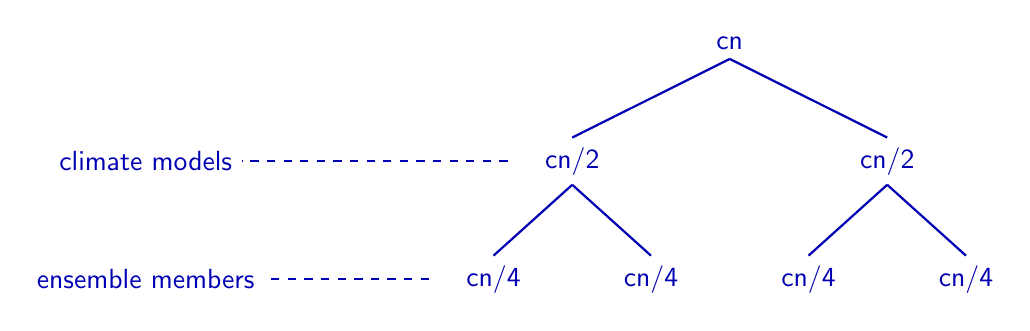
\begin{tikzpicture}[
    level/.style={sibling distance=40mm/#1},
    text=blue!70!black,
    >=latex,
    font=\sffamily
    ]

\node (z){cn}
  child {node (a) {cn/2}
    child {node  (b) {cn/4}}
    child {node (g) {cn/4}}
  }
    child {node (d) {cn/2}
      child {node  (e) {cn/4}}
      child {node (f) {cn/4}}
};

\node[left=7 of z]  (ln1) {}[no edge from this parent]
    child {node (ln2) {climate models}[no edge from this parent]
        child {node (ln3) {ensemble members}[no edge from this parent]}};

\draw[blue!70!black,dashed,thick]
    ($(a.west)+(-1em,0)$) -- (ln2.east);
\draw[blue!70!black,dashed,thick]
    ($(b.west)+(-1em,0)$) -- (ln3);

\end{tikzpicture}
\end{document}
